\documentclass[11pt]{article}
\usepackage[margin=1.15in]{geometry}
\usepackage{amsmath,amssymb,amsthm}
\usepackage{booktabs}
\usepackage{tabularx}
\usepackage{tikz}
\usetikzlibrary{positioning,arrows.meta}
\usepackage[expansion=false]{microtype}
\usepackage{enumitem}
\usepackage[colorlinks=true,linkcolor=black,citecolor=black,urlcolor=black]{hyperref}

\theoremstyle{definition}
\newtheorem{definition}{Definition}
\theoremstyle{remark}
\newtheorem{remark}{Remark}

\newcommand{\Yf}{Y_{\mathrm{formal}}}
\newcommand{\HP}{\mathrm{HP}}

\title{The Admissible Subspace:\\
Reductions, Representations, and the Counterfeit Possibilities\\
of Transformed Spaces}
\author{Flyxion\\\small Independent Researcher}
\date{September 2026}

\begin{document}
\maketitle

\begin{abstract}
\noindent
A transformation that makes a problem tractable also enlarges what can be said about it. The transformed space contains objects that are well formed there and that correspond to nothing in the system the transformation started from. Two recent papers, written in unrelated fields, treat this gap as their subject. Song et al.\ (\textit{Scientific Reports}, 2026) reduce the Kuralay--IIA wave equation to a planar Hamiltonian system and show that a formally exact solution of the reduced equations can fail to be a travelling wave of the original equation, deriving the conditions that separate the two. Li et al.\ (\textit{Nature Communications}, 2026) build a traffic-scene object detector in which the scale of observation is chosen per location from local spectral content, because a single scale everywhere destroys distinctions that a downstream operation needs. This essay states the shared structure. Reductions drop constraints, and the dropped constraints are the gates that an object in the reduced space must still pass. Lossy views produce counterfeit equivalences, and fusing views works only where their losses differ. The essay places both cases in the vocabulary of the author's holocoordinate systems (blind spaces, holonomy, quotient charts), reads admissibility as a use-indexed permission in the sense of the reversibility gate, distinguishes two kinds of counterfeit, and separates the papers' claims from its own formalization. The places where the evidence in each paper stops are listed at the end.
\end{abstract}

\section{Why a transformation makes counterfeits}

Reduction is the working method of applied mathematics. A partial differential equation is restricted to travelling waves and becomes an ordinary differential equation. A photograph is filtered and downsampled and becomes a feature map. In each case a hard object is replaced by an easier one that keeps something of the original, and analysis proceeds in the easier space.

The risk is structural. Let $X$ be the originating system, $R:X\to Y$ a reduction or representation, and $\Yf$ the set of objects that are well formed under the rules of the reduced space. It is natural to behave as though $\Yf\approx R(X)$, so that whatever is valid in $Y$ came from something in $X$. In general
\begin{equation}
  R(X)\;\subsetneq\;\Yf .
  \label{eq:strict}
\end{equation}
The transformed space has more possibilities than the system it represents. Anything in $\Yf\setminus R(X)$ is a counterfeit: it passes every test the reduced space can administer and corresponds to nothing in $X$. Nothing in $Y$ marks it as counterfeit, because the marks that would do so are the information the reduction discarded.

The essay develops this in two cases. In the first, the discarded information is an equation, and the counterfeit is a formally exact wave. In the second, the discarded information is spectral detail, and the counterfeit is an equivalence between signals that were different. The two cases are then compared, and the operation that removes counterfeits, an admissibility test, is stated in general form.

\section{A reduction that admits too much}

The Kuralay--IIA system is
\begin{equation}
  iS_t - S_{xt} - SU = 0, \qquad U_x - 2\varepsilon\,(|S|^2)_t = 0,
  \label{eq:kuralay}
\end{equation}
with $S(x,t)$ a complex envelope, $U$ a real auxiliary field, and $\varepsilon=\pm1$ setting the sign of the nonlinearity. Song et al.\ seek travelling waves in the form
\begin{equation}
  S(x,t)=\phi(\xi)\,e^{i(kx-\omega t)},\qquad U(x,t)=u(\xi),\qquad \xi=x-ct.
  \label{eq:ansatz}
\end{equation}
Substituting into the first equation gives a single complex relation,
\[
  c\phi'' + i\phi'\,[\,c(k-1)+\omega\,] + \phi\,[\,\omega(1-k)-u\,] = 0 ,
\]
which the ansatz splits into two real ones:
\begin{align}
  \text{real:}\quad & c\phi'' + [\,\omega(1-k)-u\,]\phi = 0, \label{eq:real}\\
  \text{imaginary:}\quad & [\,c(k-1)+\omega\,]\,\phi' = 0. \label{eq:imag}
\end{align}
For a nontrivial wave, $\phi'\not\equiv0$, and the imaginary equation then forces
\begin{equation}
  \boxed{\,k \;=\; 1-\frac{\omega}{c}\,}
  \label{eq:gate1}
\end{equation}
the first admissibility constraint of the paper. The second equation of the system integrates once, $u' = -2\varepsilon c\,(\phi^2)'$, and the integration constant is fixed by choosing a reference amplitude $\phi_0$ at which $u$ vanishes, giving $u=2\varepsilon c(\phi_0^2-\phi^2)$. The real equation becomes a particle in a potential,
\begin{equation}
  \phi'' = -V'(\phi),\qquad V(\phi)=\frac{\omega^2}{2c^2}\phi^2+\varepsilon\Big(\frac{\phi^4}{2}-\phi_0^2\phi^2\Big),
  \label{eq:potential}
\end{equation}
and the phase plane $(\phi,y=\phi')$ carries the conserved Hamiltonian $H=\tfrac12y^2+V(\phi)$. The rest of the paper is phase-plane geometry: equilibria at $\phi=0$ and, when $\Delta:=\phi_0^2-\omega^2/(2\varepsilon c^2)>0$, at $\phi=\pm\sqrt{\Delta}$, with $V''(0)=-2\varepsilon\Delta$ and $V''(\pm\sqrt\Delta)=4\varepsilon\Delta$.

\subsection{The constraint the phase plane does not contain}

The point that matters for this essay is where the gate~\eqref{eq:gate1} sits. It comes from the imaginary equation. The phase plane comes from the real equation. The planar system~\eqref{eq:potential} has no place in which $k$ appears; the wave number has been absorbed into a single coefficient. To see this, keep the real equation as it stands and write $\Omega:=\omega(1-k)$. The real equation alone defines a family of potentials
\begin{equation}
  V_\Omega(\phi)=\frac{\Omega}{2c}\phi^2+\varepsilon\Big(\frac{\phi^4}{2}-\phi_0^2\phi^2\Big),
  \label{eq:formal-potential}
\end{equation}
and its solutions, orbits of the planar system, are what the paper calls trajectories that exist geometrically. Setting $\Omega=\omega^2/c$ recovers Equation~\eqref{eq:potential}. The imaginary equation is exactly the statement that $\Omega$ is not free: $\Omega=\omega^2/c$.

An example fixes the idea. Take $\varepsilon=1$, $\phi_0=3/2$, $c=1$, and choose $k=0$ and $\omega=1/2$, so $\Omega=1/2$. The real equation is then perfectly satisfiable by a bright soliton: $V_\Omega''(0)=\Omega/c-2\varepsilon\phi_0^2=-4<0$, the origin is a saddle, and a homoclinic loop through it decays as $e^{-2|\xi|}$. The imaginary coefficient is $c(k-1)+\omega=-1/2\neq0$, so $\phi'$ must vanish identically. There is no such wave. It is a formally exact solution of the reduced ODE and not a solution of the equation it was reduced from.

Two refinements keep the statement accurate, and both are the essay's own working-out of the paper's equations.

First, the counterfeit in this example is the pairing of the profile with the phase, not the profile. For the same $c$, $\phi_0$, and $\Omega/c=1/2$, the admissible phase is $\omega'=\sqrt{c\Omega}\approx0.707$ and $k'=1-\omega'/c\approx0.293$, and $S=\phi(\xi)e^{i(k'x-\omega' t)}$ with that same profile does solve the system. What the phase plane cannot show is which phase belongs with the profile.

Second, the gate also removes part of the profile space. Since $\Omega=\omega^2/c\ge0$ for $c>0$, formal potentials with $\Omega/c<0$ have no admissible realization at all. Under the gate the quadratic coefficient of the potential is $\omega^2/2c^2\ge0$, and the formal space contains members the equation excludes even after relabelling.

The parameter count summarizes it. The formal space is indexed by $(\varepsilon,\phi_0,c,\omega,k)$. Only $\Omega/c$ affects the phase-plane shape, so one direction in $(\omega,k)$ is invisible to the geometry. The gate is a codimension-one submanifold of the nominal parameter space and it lives in that invisible direction.

\subsection{The gate as a section of a quotient}

The holocoordinate essay's treatment of parameter redundancy applies directly \cite{holo}. The phase plane sees a wave only through $(\varepsilon,\phi_0,\Omega/c)$. Write $\rho(\omega,k)=\omega(1-k)$ for the map from phase parameters to what the phase plane registers. Chart values then live in the quotient by $\sim_\rho$, whose fibres are the curves $\omega(1-k)=\text{const}$, and a function of the parameters descends to a function of the chart values if and only if it is constant on fibres. The wave number is not. On the fibre $\Omega=1/2$ (with $c=1$) the points $(\omega,k)=(1/2,0)$ and $(0.707,0.293)$ have different $k$, so a wave number fitted to a profile is not determined by what the phase plane distinguishes.

The gate repairs this. On each fibre with $c>0$, $\Omega>0$, and $\omega>0$, the condition $c(k-1)+\omega=0$ holds at exactly one point, $\omega=\sqrt{c\Omega}$. The gate is therefore a section $s$ of the quotient: it selects one representative from every fibre. In the holocoordinate essay a section is a choice, and the holonomy it produces (render, refit, read the parameters again) is a gauge artifact that another choice would move. Here the section is forced by the equation, and the round-trip discrepancy
\[
  \Omega_{\mathrm{rt}}(\omega,k)=d\big((\omega,k),\,s(\rho(\omega,k))\big)
\]
vanishes exactly on the gate. Admissibility, in this case, is the locus on which a render-and-refit loop returns its starting point. The quantities that survive moving a formal pair back to the gate are those that depend on the fibre alone.

\section{A second gate, and two kinds of counterfeit}

Passing the first gate makes every orbit of the phase plane an exact solution of the system, periodic and unbounded orbits included. The paper's second gate concerns solitary waves. A localized wave has a far-field background $\phi_\infty=\lim_{\xi\to\pm\infty}\phi(\xi)$, and the paper requires three conditions jointly: the background is an equilibrium, $V'(\phi_\infty)=0$; the orbit energy equals the potential at that equilibrium, $H(\phi_\infty,0)=V(\phi_\infty)$; and the equilibrium is a saddle, $V''(\phi_\infty)<0$. A centre supports no extended orbit at its own energy, since the level set collapses to a point, and a saddle's stable and unstable manifolds coincide on the energy level and form the separatrix, homoclinic when $\phi_\infty=0$ and heteroclinic when the two saddles $\pm\sqrt\Delta$ are joined.

The classification that results is compact (Table~\ref{tab:cases}). Bright solitons need the origin to be a saddle, $V''(0)=\omega^2/c^2-2\varepsilon\phi_0^2<0$, which requires $\varepsilon>0$ and $\Delta>0$. Dark solitons need saddles at $\pm\sqrt\Delta$, $4\varepsilon\Delta<0$, which requires the defocusing sign. For $\varepsilon<0$ the discriminant is $\Delta=\phi_0^2+\omega^2/(2|\varepsilon|c^2)>0$ automatically. The paper's numerical values ($c=1$, $\phi_0=1.5$; $\omega=1$ for cases 1, 3, and 4 and $\omega=3$ for case 2) reproduce these entries, and the arithmetic checks: $\Delta=1.75,\,-2.25,\,2.75$ for cases 1, 2, 3.

\begin{table}[t]
\centering
\small
\begin{tabular}{@{}clll@{}}
\toprule
Case & $\varepsilon$, $\Delta$ & Equilibria & Admissible waves \\
\midrule
1 & $>0$, $>0$ & saddle at 0, centres at $\pm\sqrt\Delta$ & homoclinic loop: bright soliton \\
2 & $>0$, $\le0$ & single centre at 0 & periodic orbits only \\
3 & $<0$, $>0$ & centre at 0, saddles at $\pm\sqrt\Delta$ & heteroclinic pair: dark soliton \\
4 & $=0$ & single centre (quadratic) & linear periodic waves only \\
\bottomrule
\end{tabular}
\caption{The four regimes of the paper's Table~1, after the first gate.}
\label{tab:cases}
\end{table}

The paper says that an orbit which fails the criterion ``exists geometrically but is physically incompatible.'' The essay distinguishes two ways of failing, because they are different kinds of object.

\begin{definition}[Type I and Type II counterfeits]
A \emph{Type I counterfeit} satisfies the reduced representation and violates a constraint of the original system that the reduction dropped. It is not a solution. A \emph{Type II counterfeit} is a genuine solution that is presented as an object of a type it does not have.
\end{definition}

The formal soliton with $k=0$, $\omega=1/2$ is Type I: the imaginary equation, dropped in passing to the phase plane, rules it out. A candidate presented as a soliton on background $\phi_\infty$ but whose energy differs from $V(\phi_\infty)$, or whose background sits at a centre, is Type II. It solves the system, since it is an orbit of the planar system with the first gate satisfied, but it is a periodic wave presented as a soliton. The paper's phrase ``incompatible with the original PDE'' applies literally to the first and loosely to the second. The distinction matters for what the test is doing: gate one certifies membership in $R(X)$, and gate two certifies membership in a named class within it.

Figure~\ref{fig:ladder} shows the resulting ladder,
\[
  \text{representable}\;\supsetneq\;\text{geometrically realizable}\;\supsetneq\;\text{dynamically consistent}\;\supsetneq\;\text{physically admissible},
\]
with each rung defined by a test the previous rung cannot perform.

\begin{figure}[t]
\centering
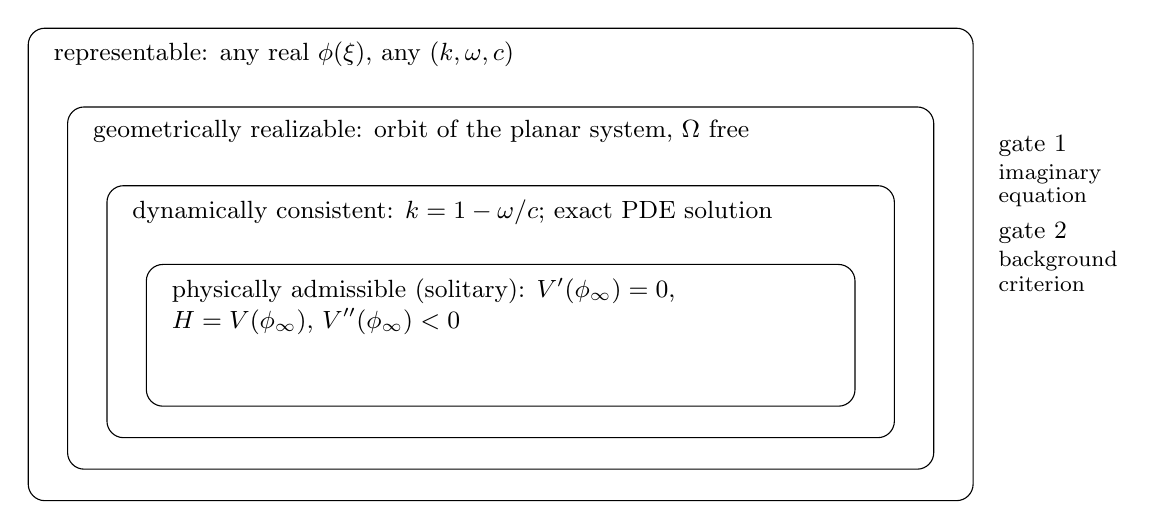
\begin{tikzpicture}[every node/.style={font=\small}]
  \draw[rounded corners=6pt] (0,0) rectangle (12,6.0);
  \node[anchor=north west] at (0.2,5.95) {representable: any real $\phi(\xi)$, any $(k,\omega,c)$};
  \draw[rounded corners=6pt] (0.5,0.4) rectangle (11.5,5.0);
  \node[anchor=north west] at (0.7,4.95) {geometrically realizable: orbit of the planar system, $\Omega$ free};
  \draw[rounded corners=6pt] (1.0,0.8) rectangle (11.0,4.0);
  \node[anchor=north west] at (1.2,3.95) {dynamically consistent: $k=1-\omega/c$; exact PDE solution};
  \draw[rounded corners=6pt] (1.5,1.2) rectangle (10.5,3.0);
  \node[anchor=north west,align=left] at (1.7,2.95) {physically admissible (solitary): $V'(\phi_\infty)=0$,\\ $H=V(\phi_\infty)$, $V''(\phi_\infty)<0$};
  \node[anchor=west] at (12.2,4.5) {gate 1};
  \node[anchor=west,font=\footnotesize] at (12.2,4.15) {imaginary};
  \node[anchor=west,font=\footnotesize] at (12.2,3.85) {equation};
  \node[anchor=west] at (12.2,3.4) {gate 2};
  \node[anchor=west,font=\footnotesize] at (12.2,3.05) {background};
  \node[anchor=west,font=\footnotesize] at (12.2,2.75) {criterion};
\end{tikzpicture}
\caption{The admissibility ladder for travelling waves of the Kuralay--IIA equation. Gate 1 removes Type I counterfeits. Gate 2 removes Type II counterfeits within the solitary-wave class.}
\label{fig:ladder}
\end{figure}

\section{The general schema}

The Kuralay case has a structure that does not depend on it. Suppose the originating system $X$ is defined by constraints $C_1,\dots,C_m$. A reduction uses a subset $C_S$ of them to build the reduced space and disposes of the rest, $C_D$, by absorbing them into parameters or by not representing them. Then
\begin{equation}
  \Yf=\{y:\,C_S(y)\},\qquad R(X)\;\subseteq\;\{y\in\Yf:\,C_D(y)\}\;\subsetneq\;\Yf .
  \label{eq:schema}
\end{equation}
Define the admissibility predicate $A:\Yf\to\{0,1\}$ by $A(y)=1$ exactly when $C_D(y)$ holds. It is a necessary test, not a reconstruction. Reductions generally lose information, so $R(X)$ may be smaller than $A^{-1}(1)$: passing the test does not certify that $y$ came from a particular state of $X$. The imaginary equation is such a case. It certifies that a profile-phase pair generates a solution and says nothing about how the solution arose. The formalization separates two things that are easy to run together: necessary admissibility tests, and perfect reconstruction of provenance.

Two consequences follow.

\emph{Admissibility conditions are the memory of the originating system.} They are exactly the constraints the reduction dropped, so they cannot be read off from the reduced representation and must be carried from the origin. A phase portrait, however carefully classified, does not contain the equation that says which portraits are real.

\emph{Admissibility is relative to what the reduction fixes from outside.} The integration constant in $u=2\varepsilon c(\phi_0^2-\phi^2)$ is not determined by the differential equation. The paper fixes it by choosing a reference amplitude. The classification in Table~\ref{tab:cases} is therefore a classification relative to that datum, and it depends on the ansatz~\eqref{eq:ansatz} with constant $k$ and $\omega$ and a real $\phi$. Within that class the paper's completeness claim stands. Outside it, for example with a phase that varies with $\xi$, the gates say nothing.

\subsection{Gates that are earned}

The gates of Sections~2 and 3 are checked: a candidate $y\in\Yf$ is given, the predicate $A$ is evaluated, and a verdict returns. A different kind of gate is searched. Candidates are generated in a fixed order and refused until one passes, and what is then admitted is downstream of the search. The clearest instance is a hash-below-target predicate. Let $\mathsf h$ be a hash function, $x$ a fixed structure, and $T_d$ a threshold set by a difficulty $d$, and define
\[
  A_d(n)=\mathbf 1\{\mathsf h(x\Vert n)<T_d\},\qquad n^{\star}=\min\{n\ge0:\ A_d(n)=1\}.
\]
The pair $w=\big(n^{\star},\mathsf h(x\Vert n^{\star})\big)$ is a witness, and the admissibility of the artifact $(x,w)$ is certified by a verifier $V(x,w)$ that costs one hash evaluation. Four properties bear on the schema.

\emph{Asymmetry.} Verifying costs one evaluation. Producing a witness costs, if $\mathsf h$ behaves as a random function and each trial passes with probability $p_d$, an expected $1/p_d$ evaluations, and tightening the gate lowers $p_d$. Admission is unforgeable by cost, not by information: a counterfeit is an object presented without a satisfying witness, and a single check detects it.

\emph{Canonical witness.} Taking the minimum makes the witness unique. The set of satisfying $n$ plays the role of a fibre in Section~2.2, and $n^{\star}$ is a section of it, selected by minimality and not by an equation. Any satisfying witness verifies, but only the minimal one makes the artifact reproducible: a second party with the same $x$, $d$, and downstream rule regenerates not merely a valid witness but the same one, and therefore the same artifact.

\emph{Provenance.} Equation~\eqref{eq:schema} separates a necessary test from reconstruction of provenance. Here the artifact carries its own certificate, so for artifacts of the form $(x,w)$ the inclusion $R(X)\subseteq A^{-1}(1)$ holds with equality by construction. The certificate shows that a passing candidate was found. It does not show who searched or with what effort, which is a further assumption about the hash.

\emph{Lineage.} If the parameters of a downstream object are computed from the witness, the object depends on the search in the sense of the reversibility gate's dependency lineage \cite{revgate}. Change $x$ or $d$ and every dependent quantity changes with them, so rollback is well defined, and the dependency is explicit and not inferred.

One design consequence is worth stating. The cost of admission can be carried into the object as a parameter, and nothing requires that cost to be rendered as more activity. A design may render it as inertia, so that a tighter gate yields a slower and heavier object, and the parameter then records what was spent to admit it. In the atlas of Section~10 it would be one more component of the coordinate, beside the resolution field. Work earns the witness, and the witness earns the object.

\section{A transformation that destroys distinctions}

The second case does not drop an equation. It drops detail. Li et al.\ build a one-stage detector, the Frequency-Oriented Adaptive Detector (FAD), around a conflict they take from Fourier analysis. A dilated convolution with dilation $D$ places its taps $D$ pixels apart. Its frequency response is that of the undilated kernel compressed by a factor $D$, $W_D(f)=W(Df)$, and the highest frequency it can represent without aliasing falls from $1/2$ to $1/(2D)$ cycles per pixel. Increasing the dilation buys context, since the receptive field of a $K\times K$ kernel is $(K-1)D+1$, and pays for it in high-frequency sensitivity. A single global dilation therefore sets one exchange rate between context and detail for every location in the image.

\subsection{Aliasing as counterfeit}

The counterfeit mechanism is cleanest in the downsampling that multi-scale detectors perform. Sampling at half rate maps a component at frequency $f\in(1/4,1/2)$ to $1/2-f$. Concretely, sampling every second pixel of $\cos(2\pi\,0.1\,n)$ gives $\cos(2\pi\,0.2\,m)$, and sampling every second pixel of $\cos(2\pi\,0.4\,n)$ gives $\cos(2\pi\,0.8\,m)=\cos(2\pi\,0.2\,m)$, the same sequence. A smooth region and a fine texture have become indistinguishable. The coarse representation now contains what looks like genuine low-frequency structure that originated as high-frequency content. It is a member of the reduced space that cannot be traced back to the structure it came from. In the notation of Section~1, two distinct states $x_1\neq x_2$ of $X$ satisfy $f(x_1)=f(x_2)$, and no downstream map $g$ can tell them apart, because $g\circ f$ has the same value on both.

The paper's account of why this matters for detection is its similarity analysis. Fusing a coarse high-level feature map with a fine map by bilinear upsampling produces intra-category inconsistency, where the parts of one object (a wheel and a window) receive dissimilar features, and boundary displacement, where smoothing moves edges. They quantify both with intra-category and inter-category similarity and their difference, the similarity margin, illustrated on two KITTI examples (Fig.~1 of the paper), and they attribute both defects to a spectral imbalance across locations.

\subsection{The admissible dilation at a point}

The paper's remedy for the extraction stage is an adaptive dilation rate: the fixed $D$ is replaced by a per-pixel $\hat D(p)$,
\begin{equation}
  Y(p)=\sum_{i=1}^{K\times K}W_i\,X\big(p+\Delta p_i\,\hat D(p)\big),
  \label{eq:adaptive}
\end{equation}
with $\hat D$ predicted by a convolutional layer followed by a ReLU. To decide what $\hat D(p)$ should be, they define the high-frequency power
\begin{equation}
  \HP(p)=\sum_{(u,v)\in\mathcal H^{+}_{\hat D(p)}}\big|X_F^{p,s}(u,v)\big|^2,
  \label{eq:hp}
\end{equation}
the local spectral power above the cutoff $1/(2\hat D(p))$ that the chosen dilation cannot represent, computed from a window of size $s$ around $p$. The quantity is the detail that a given dilation would discard. The paper's objective is to maximize the total receptive field minus the total discarded power, $\theta=\max_\theta\sum_p\big(\mathrm{RF}(p)-\HP(p)\big)$. Because $\HP$ is discrete and non-differentiable, they implement it through a dual heuristic: raise the dilation at pixels in the lowest quartile of high-frequency power and suppress it at pixels in the highest quartile. Their Figure~5 shows the learned relation, with lower dilations assigned to high-frequency regions such as object boundaries.

This can be restated as a gate. Since raising $D$ lowers the cutoff, $\HP(p;D)$ is nondecreasing in $D$. Define the admissible dilations at $p$ for a tolerance $\tau$ on discarded power:
\begin{equation}
  \mathcal D(p)=\{D\ge1:\ \HP(p;D)\le\tau\}=[\,1,\,D_{\max}(p)\,],\qquad
  D^{*}(p)=D_{\max}(p).
  \label{eq:admissible-dilation}
\end{equation}
The interval is nested in $D$, and a location whose spectrum has more power above every cutoff has a smaller $D_{\max}$. So the rule the paper reports empirically, small dilation where high-frequency power is large, is what Equation~\eqref{eq:admissible-dilation} predicts. This is the essay's reformulation of the paper's objective as a constrained problem, not the paper's own formulation, and the two share a monotone structure without being equivalent in general.

The gate here differs from the Kuralay gate in one respect that is central to the comparison. The Kuralay gate, $k=1-\omega/c$, is a fixed submanifold of the parameter space fixed by the equation. The dilation gate is a field. The set of admissible operations $\mathcal D(p)$ varies from point to point with what is being observed. The observed signal helps decide how it may be observed.

\section{Resolution as a field}

Generalize the dilation gate. Let $I(x,r)$ be the information retained around $x$ when the field is observed at scale $r$, $C(x,r)$ the contextual coverage that scale provides, and $K(r)$ its computational cost. A scale of observation that is appropriate at $x$ solves
\begin{equation}
  R^{*}(x)\;=\;\arg\max_{r}\Big[\alpha(x)\,I(x,r)+\beta(x)\,C(x,r)-\lambda K(r)\Big].
  \label{eq:resolution}
\end{equation}
The paper's objective is a special case: $C$ is the receptive field, $I$ is the negative of the discarded power, both weights equal one, there is no cost term, and the optimum is approximated by the quartile heuristic. Equation~\eqref{eq:resolution} is the essay's abstraction, and its point is the argument $x$. Resolution becomes a field $R:M\to\mathbb R_{+}$ over the observed domain, with weights that may vary along it, and the interesting object is that field and its gradient. A large gradient of $R$ means that a small movement through the represented space changes how finely the system must inspect it. Boundaries are such places. An edge is not only something represented. It changes the conditions under which the representation should be built.

The rest of the architecture spends its parameters on the same idea in other forms. The adaptive kernel splits each kernel into its mean $\bar W$ (a low-pass filter) and its residual $\hat W=W-\bar W$ (which carries local variation) and reweights them, $W=\lambda_l\bar W+\lambda_h\hat W$, with $\lambda_l,\lambda_h$ predicted per channel from globally pooled features. A frequency selection stage splits features into four octave bands and recombines them with spatial selection maps $A_b(i,j)$. Cross-scale contribution allocation fuses features from several levels with per-position weights $\alpha,\beta,\gamma$ that sum to one, $y_{ij}=\alpha_{ij}x^{1\to l}_{ij}+\beta_{ij}x^{2\to l}_{ij}+\gamma_{ij}x^{3\to l}_{ij}$. That last constraint is a competition: at each position the scales share a fixed budget of contribution, which is a soft assignment of resolution to location.

\section{Complementary forgetting}

The fusion mechanism raises the second question: what can be done after a distinction has been destroyed. The answer from Section~5 is nothing, at that point. The paper's design follows from accepting this.

\begin{remark}[Fusion cannot recover what a branch has discarded]
If a branch $f$ satisfies $f(x_1)=f(x_2)$ for $x_1\neq x_2$, then no map $g$ applied to $f(X)$ alone can separate $x_1$ from $x_2$. Distinctions must be preserved by a different branch before the collapse.
\end{remark}

Represent the views as maps $V_i:X\to Y_i$, each with an equivalence relation $x\sim_i x'$ iff $V_i(x)=V_i(x')$. A joint representation separates $x$ and $x'$ unless every view identifies them, so the pairs it fails to separate are those in $\bigcap_i\sim_i$. For linear views this is the condition $\bigcap_i\ker V_i=\{0\}$. An idealized case makes it concrete: a low-pass-and-decimate view has as its kernel the signals confined to the band above the cutoff, a high-pass view has as its kernel the signals confined to the band below it, and the two kernels intersect trivially. Each view forgets something, the forgetting is not the same forgetting, and the pair together forget nothing. The idealization is the essay's and real learned filters do not achieve it. In the vocabulary of the holocoordinate essay \cite{holo}, the condition is multidifference completeness: with $\mathcal N_i=\ker V_i$ the blind space of view $i$ and $\mathcal N=\bigcap_i\mathcal N_i$ the joint blind space, the family is complete if and only if $\mathcal N=\{0\}$, equivalently if and only if the frame operator $S=\sum_iV_i^{*}V_i$ is positive definite. Completeness is weaker than holography: a family can register every difference while no single view separates the states it needs to separate. For the ideal band split, with $P_L$ and $P_H$ orthogonal projections onto complementary spectral bands, $S=P_L+P_H=\mathrm{id}$ and the observational condition number is one. With channel weights $\lambda_l,\lambda_h$ on the two views, $S=\lambda_l^2P_L+\lambda_h^2P_H$ and $\kappa_{\mathrm{obs}}=\max(\lambda_l/\lambda_h,\lambda_h/\lambda_l)$. Under the idealization, the ratio that the paper's adaptive kernel predicts from the input is the condition number of the two-band view, and it controls how strongly noise in the weaker band is amplified in reconstruction, since the least-squares error is bounded by $\|\eta\|/\sigma_{\min}$. The paper's kernel decomposition splits weights into a mean and a residual, which are not orthogonal band projections, so the identity is a property of the idealization and not of the network. Conditioning also depends on the weights chosen, and should be reported with them.

FAD's high-pass adaptive filter (HAF) is built on this structure. The filters are predicted from the initially fused feature $Z^l$, but they are applied to the low-level feature $X^l$, which still holds the high-frequency content: $\tilde X^l_{i,j}=X^l_{i,j}+\sum_{p,q}\hat W^{l,p,q}_{i,j}X^l_{i+p,j+q}$, with the kernels obtained as the identity minus a softmax low-pass kernel. Boundary information is drawn from the branch that kept it. The low-pass adaptive filter and the offset generator, which resamples toward locally similar features guided by cosine similarity to the eight neighbours, work on the other side of the ledger: they enforce continuity within a region. Low frequencies help answer which pixels belong together. High frequencies help answer where the region stops. Continuation without distinction smears, and distinction without continuation fragments, so the representation needs both operators and a rule for weighing them.

The paper's ablation is consistent with partly overlapping remedies. On KITTI, mean average precision rises from 87.7 for the baseline to 89.3 with the frequency dynamic convolution, 90.2 with the fusion module, and 90.9 with both. The separate gains, 1.6 and 2.5 points, sum to more than the joint gain of 3.2. That is what one would expect if the two modules recover partly the same lost distinctions, but the ablation does not test the mechanism, and other explanations exist.

\section{Two gates, one structure}

The papers concern different things, and their arguments have the same shape (Table~\ref{tab:compare}).

\begin{table}[t]
\centering
\small
\begin{tabularx}{\textwidth}{@{}p{2.6cm}XX@{}}
\toprule
 & Kuralay--IIA waves & Frequency-oriented detector \\
\midrule
Originating system & the PDE~\eqref{eq:kuralay} & the image and its spectrum \\
Transformation & travelling-wave reduction to a planar ODE & dilation, downsampling, fusion \\
What it forgets & the imaginary equation; the wave number as an independent variable & high-frequency detail above the cutoff \\
Counterfeit & Type I: a formal orbit that is no solution. Type II: a solution mislabelled as a soliton & aliased equivalence: distinct signals identified \\
Gate & $k=1-\omega/c$; then saddle background and matched energy & $\HP(p;D)\le\tau$, per location \\
Gate depends on & the equation and the datum $\phi_0$ & the local spectrum of the input \\
Remedy for lost information & carry the dropped equation & preserve detail in a second branch \\
\bottomrule
\end{tabularx}
\caption{The two cases compared.}
\label{tab:compare}
\end{table}

In both, the object that goes wrong is not a mistake in the reduced space. Every element of $\Yf$ is well formed there. In both, the test that catches the problem refers back to the originating system, an equation in the first case and a spectrum in the second, so it cannot be performed inside the representation. In both, a naive reading of the transformed space (every orbit is a wave, every coarse feature is real structure) transports a property of $Y$ back into a claim about $X$ that $X$ does not support.

The difference is in what the gate depends on. The wave gate is fixed by the equation. The detector's gate is computed from the data, which is why the second case gives the essay its resolution field. That difference indicates a way to classify admissibility tests: static gates (a fixed submanifold of parameters, decided by the system's constraints) and dynamic gates (a set of allowed operations recomputed from the current state of the observed field).

The two papers do not support one another, and the essay does not claim they do. They are independent instances of a structure that recurs. The closest earlier statements in this series are that a residual, an error, or a refusal is intelligible only relative to the continuations available downstream (\emph{When Failure Becomes a Signal}, \emph{The Unequal Error}, \emph{The Waste Is in the Boundary}). Two of the author's own frameworks bear on it directly: the holocoordinate atlas supplies the vocabulary of blind spaces, quotients, and holonomy, and the reversibility gate supplies the separation of a status from a permission. The present statement is narrower and more mechanical: a transformation enlarges the apparent space of possibilities, and admissibility is the operation that returns properties of the transformed space to the constraints of the space it came from.

\section{Existence is not permission}

The reversibility gate \cite{revgate} separates two properties that are routinely merged. A claim's readiness for judgment belongs to the claim and its declared evidential procedure. An action's permissibility belongs to the action: its reversibility, its delay sensitivity, and its claim-relative losses, evaluated against a background response $B$. The same claim can sit beneath one action that is required and another that is forbidden.

The structure carries over to representations. Well-formedness in the reduced space is the analogue of maturity: it is settled by the reduced space's own procedure. Whether the object may be carried into a claim about the originating system is a further question, and its answer depends on the use. Admissibility is therefore indexed by a pair (object, use), not by the object alone. The formal soliton of Section~2 with $k=0$, $\omega=1/2$ is permitted as a statement about the ODE, a homoclinic loop with decay rate $\sqrt{2\varepsilon\phi_0^2-\Omega/c}=2$, and forbidden as a statement about the PDE. A Type I counterfeit is an object whose use in $Y$ is permitted and whose use in $X$ is forbidden.

Four features of the gate sharpen the essay's binary tests.

\emph{Margins.} The gate returns forbid, permit, or require, with a permit band of genuine underdetermination between two margins. The tolerance $\tau$ in Equation~\eqref{eq:admissible-dilation} plays that role. Dilations with discarded power far below $\tau$ are safe, those far above are forbidden, and in between the verdict depends on the margin chosen. A binary gate hides the band.

\emph{Background dependence.} The verdict on an addition depends on what is already in $B$. The admissibility of a coarsening depends likewise on what else is in place: with a fine branch retaining high-frequency detail, the marginal loss from a larger dilation on the coarse branch is smaller, and a dilation that would be forbidden alone can become permitted. This is the essay's inference from the gate's structure. The paper does not test it, and its ablation does not vary the dilation tolerance with the fusion module present.

\emph{Irreversibility.} The gate charges an action for the future options it forecloses, and scores abstention on the same terms as any other response. Coarsening is irreversible in this sense, since the distinctions it merges cannot be recovered downstream (Section~5), and the information term $I(x,r)$ in Equation~\eqref{eq:resolution} is an option-loss term. The two-branch design is a reversible hedge: the coarse operation proceeds while a second branch keeps the option of detail alive.

\emph{Four operations.} When a counterfeit has already been used, the gate's taxonomy of corrections applies. A Type II counterfeit has a sound profile and a contaminated phase label, and the correction is repair: keep the profile and its fibre-only consequences (amplitude, width, decay rate) and replace the phase pair by the gate's section. A Type I counterfeit used to derive further quantities calls for retraction of its warrant and rollback of its dependents, with repair for those that depended only on the fibre. Aliased features admit none of these from the coarse representation alone, because it carries no record of which components were aliased. Repair needs an independent premise, and the fine branch supplies it. This is the fusion principle of Section~7 seen from the side of correction.

\section{An enriched atlas with a resolution field}

The holocoordinate essay defines an enriched atlas $\mathfrak H=\{(U_\alpha,\phi_\alpha,\sigma_\alpha,T_{\beta\alpha},\varepsilon_\alpha)\}$ and four properties shown to be logically independent: multidifference completeness (M), strong holography (H), transition consistency (C), and holonomy triviality (V) \cite{holo}. The two cases of this essay bear on that construction in four ways.

\paragraph{A resolution field.} Both cases add a component the atlas does not carry: the scale at which the neighbourhood of a state must be observed. Let $\sim$ record the distinctions to be preserved and $\sigma_r$ be a signature at scale $r$. Define the required resolution
\[
  r^{*}_{\sim}(x)=\text{the coarsest } r \text{ for which } \sigma_r \text{ is strongly holographic with respect to } \sim \text{ near } x.
\]
Equation~\eqref{eq:resolution} is the relaxed form in which a trade-off replaces the constraint, and the dilation gate is a further relaxation with a tolerance. An observation is then specified by where, relative to what, at what scale, and preserving which distinctions, the last being $\sim$. The enriched coordinate becomes
\begin{equation}
  \mathrm{HC}(e)=\big(\phi_\alpha(e),\,T_{\beta\alpha},\,r_\alpha(e)\big),\qquad \mathcal A=\{(U_\alpha,\phi_\alpha,r_\alpha)\},
  \label{eq:holocoord}
\end{equation}
where the last component is this essay's addition. A coordinate says where to look. A coordinate with a resolution field also says how looking there must differ from looking elsewhere.

\paragraph{Transitions between scales are not invertible.} The classical atlas requires $T_{\alpha\beta}=T_{\beta\alpha}^{-1}$. A transition from a fine chart to a coarse one has no inverse: the aliasing example of Section~5 gives two states with the same coarse image. The atlas acquires a direction. Chains of coarsening can satisfy the cocycle condition, since a factor of two followed by a factor of two can equal a factor of four for matched filters, while refinement needs a finer chart to be consulted. A round trip fine, coarse, fine, through any upsampler $U$, has holonomy discrepancy $\Omega(x)=d\big(\phi_f(x),\,U\,T\,\phi_f(x)\big)$, positive for every state with content in the discarded band.

This gives three kinds of holonomy in the holocoordinate vocabulary. \emph{Topological} holonomy is the winding of the circle example there, which recoordinatizing cannot remove. \emph{Gauge} holonomy comes from parameter redundancy and vanishes in the quotient chart; the Kuralay round trip of Section~2.2 is of this kind, and it vanishes on the gate. \emph{Lossy} holonomy is the round trip through a coarser chart, removable only by identifying states the fine chart distinguishes. Aliasing is lossy holonomy.

\paragraph{Realizability is a fifth property.} Properties (M), (H), (C), and (V) concern the values a chart takes on states. None of them concerns values that the chart's rules regard as well formed but that no state takes. Call (R) the condition that the feature space of a chart, the set of values its rules accept, equals $\phi_\alpha(U_\alpha)$. It is independent of the four: on $X=[0,1]$ the chart $\phi=\mathrm{id}$ into $\mathbb R$ has $D\phi=1$, an injective signature, no transitions, and no loops, so it satisfies (M), (H), (C), and (V), while every value outside $[0,1]$ is accepted and corresponds to no state. The gates of this essay are conditions that cut $V_\alpha$ down toward $\phi_\alpha(U_\alpha)$, which is to say that they are tests for (R).

\paragraph{Growth.} The growth rule adds a coordinate $z$ when a residual is structured with respect to it, $\mathbb E[P\mid\phi,z]\neq\mathbb E[P\mid\phi]$. In detector terms, a residual of the coarse branch that is structured with respect to a fine coordinate is reduced by adding it, by the residual-reduction identity of the holocoordinate essay. That is the population-level criterion for when a second view earns its place. The detector's ablation is consistent with it and does not test it.

\section{Where the evidence stops}

\begin{itemize}[leftmargin=1.6em,itemsep=2pt]
  \item \textbf{The Kuralay paper is an unedited manuscript.} It is marked article in press, with the note that errors may remain. The algebra above was rechecked against its equations and agrees, including the entries of its Table~2, but the text may change before publication.
  \item \textbf{Admissibility is relative to the ansatz.} The characterization is complete for waves of the form~\eqref{eq:ansatz}: real amplitude, constant $k$ and $\omega$. The dark soliton it finds is a heteroclinic connection from $-\sqrt\Delta$ to $+\sqrt\Delta$ through $\phi=0$, so its intensity dips to zero. Grey profiles, which need a phase that varies with $\xi$, are outside the ansatz and not excluded by the equation.
  \item \textbf{The numerical validation tests the phase plane, not the PDE.} The tables confirm equilibrium types and the profiles confirm that the integrator conserves $H$ to $10^{-10}$. Substituting the reconstructed $S$ and $U$ back into the original system is not reported in the text. Condition (ii) of the background criterion, $H=V(\phi_\infty)$, follows from condition (i) together with convergence of the orbit to the equilibrium, so it works as a check on a proposed solution and not as an independent restriction.
  \item \textbf{Claims beyond the case studied are asserted.} Extension to perturbed variants, to Benney-type and Yajima--Oikawa models, and statements about stable intensity dips are not demonstrated, and stability is listed as future work.
  \item \textbf{FAD's mechanism is illustrated more than isolated.} The similarity analysis is shown on two examples, and Figure~5 shows the learned dilation trend. The main-text ablation treats the frequency dynamic convolution as a whole, so the contribution of the per-pixel dilation, apart from the adaptive kernel and the frequency selection, is not separated there. The dilation objective adds a receptive field in pixels to a spectral power, quantities in different units, and it is implemented through a rank-based surrogate.
  \item \textbf{The comparisons are narrower than the claims.} FAD reports 90.9 mAP on KITTI with 8.77\,M parameters, and its GFLOPs, 39.7, exceed those of the single-stage YOLO variants it is compared with (21.5 to 28.7) although they are below the transformer baseline. It runs at 57.6 frames per second against 66 to 85 for the recent YOLO models in the paper's KITTI table, and it is not best in every class and difficulty cell. The five-run mean is 90.5 with standard deviation 0.25. The reported interval, 90.3 to 90.7, matches a normal approximation, and with five runs a Student interval would be a little wider, roughly plus or minus 0.3. On the in-vehicle platform the paper reports 35.14 frames per second and 28.5\,ms latency, with only the qualitative statement that the effect on mAP was limited.
  \item \textbf{Assumptions about the spectrum.} The design rests on the premise that environmental noise is mainly low frequency and object detail mainly high frequency. The authors note that performance depends on the quality of the frequency decomposition, which may degrade under extreme lighting or weather.
  \item \textbf{The formalization is the essay's.} The schema~\eqref{eq:schema}, the counterfeit types, the constrained dilation gate~\eqref{eq:admissible-dilation}, the resolution functional~\eqref{eq:resolution}, the band-split conditioning identity, and the resolution field of Equation~\eqref{eq:holocoord} are the essay's constructions, offered to make a shared structure explicit. The holocoordinate results it borrows are stated there under smoothness hypotheses that a discretized feature map does not satisfy; the identities used here are exact only for linear views and idealized band projections.
  \item \textbf{The searched gate is the essay's own pattern.} Neither paper contains one. The cost statement assumes the hash behaves as a random function, and the certificate establishes that the predicate holds, not that any particular effort was made.
  \item \textbf{The reversibility-gate reading is an analogy.} No loss functions are estimated. The claims about margins, background dependence, and option loss describe how the gate's structure would apply, and neither paper tests them.
\end{itemize}

\section{Conclusion}

A transformation is a bargain. It buys tractability by giving up something, and what it gives up is exactly what would have let a reader of the transformed space tell a real object from a counterfeit. The Kuralay reduction gives up an equation and returns orbits that look like waves and are not. The detector's downsampling gives up detail and returns features that look like structure and are aliases. In both, the repair is not a better reading of the transformed space, because the information needed is not there. It is a test that goes back to what the transformation left behind, and, in the detector's case, a second view whose losses are not the first view's losses.

The general form is the paper-independent proposition:
\begin{quote}
\emph{Existence in the transformed space does not entail admissibility in the originating system. The constraints that decide admissibility are the ones the transformation dropped, and they must be carried from the origin or preserved in a second representation.}
\end{quote}
Some gates can be earned by search and certified by a cheap check, which lets the admitted object carry its own provenance. Admissibility is also indexed by use: the same formal object is permitted as a statement about the reduced space and forbidden as a statement about the original. The resolution of the detector adds a second lesson, about scale: there is no universally correct scale of observation, and the appropriate scale at a point depends on the distinctions that must be preserved there.

\begin{thebibliography}{9}
\bibitem{song2026} H.~Song, L.~Zhang, X.~Wang, X.~Jin and Y.~Tong, Geometric admissibility conditions for travelling-wave solitons in the Kuralay--IIA equation, \emph{Sci.\ Rep.}\ (2026), article in press, \url{https://doi.org/10.1038/s41598-026-62850-3}.
\bibitem{li2026} Z.~Li, T.~Gao, S.~Li, T.~Chen, Y.~An, Y.~Wen and T.~Lei, Frequency-oriented adaptive real-time object detector for cluttered traffic scenes, \emph{Nat.\ Commun.}\ \textbf{17}, 9787 (2026), \url{https://doi.org/10.1038/s41467-026-76346-1}.
\bibitem{holo} Flyxion, \emph{Holocoordinate Systems: Multidifference Observation, Transition Structure, and Residual Growth in Enriched Atlases}. Unpublished essay, 2026.
\bibitem{revgate} Flyxion, \emph{The Reversibility Gate: Evidence, Delay, and Action Under Unsettled Claims}. Unpublished essay, 2026.
\bibitem{shannon} C.~E.~Shannon, Communication in the presence of noise, \emph{Proc.\ IRE} \textbf{37}, 10--21 (1949).
\bibitem{guckenheimer} J.~Guckenheimer and P.~Holmes, \emph{Nonlinear Oscillations, Dynamical Systems, and Bifurcations of Vector Fields} (Springer, 1993).
\end{thebibliography}

\end{document}
